\documentclass[border=9pt]{standalone}
\usepackage[fontset=fandol]{ctex}
\usepackage{amsmath,amssymb,tikz}
\usetikzlibrary{arrows.meta,calc,decorations.pathmorphing}
\tikzset{arr/.style={-{Stealth[length=2mm]},semithick}}
\begin{document}

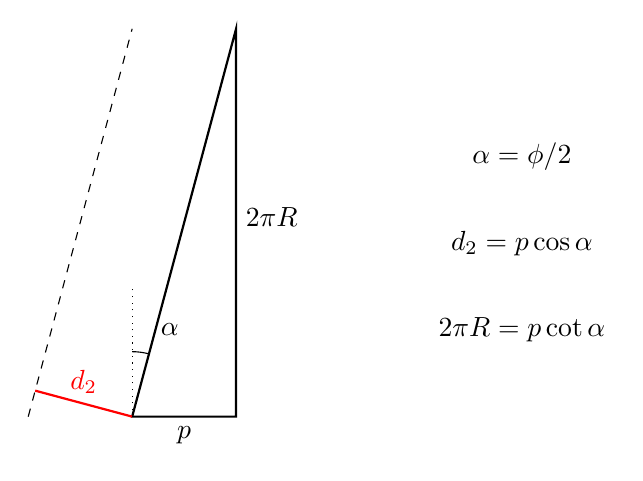
\begin{tikzpicture}[scale=1.1]
\draw[thick](0,0)--(1.2,0)--(1.2,4.478)--cycle;
\node[below]at(.6,0){$p$};\node[right]at(1.2,2.3){$2\pi R$};
\draw[dashed](-1.2,0)--(0,4.478);
\draw[red,thick](0,0)--(-1.1196,.3)node[midway,above]{$d_2$};
\draw[dotted](0,0)--(0,1.5);
\draw (0,.75)arc(90:75:.75);\node[right]at(.22,1){$\alpha$};
\node at(4.5,3){$\alpha=\phi/2$};\node at(4.5,2){$d_2=p\cos\alpha$};
\node at(4.5,1){$2\pi R=p\cot\alpha$};
\end{tikzpicture}
\end{document}
